\section{绪论}
\par 随着计算机技术和网络技术的发展,人们将计算机和网络应用在自己的工作学习娱乐生活中的场景越来越高,尤其是在流
量资费下降和移动手机、个人计算机日渐普及的社会背景下,人们可以轻易的制造、获取、传播文件资源,在这一过程中,
有限的终端存储空间越来越不能满足人们日益增的存储需求,而且终端设备具有强大的移动属性,因此数据损坏的风险也不
能够忽视\cite{r5,r6,r7}。因此本文设计开发了一套云端的存储系统,可以帮助人们解决移动终端存储空间不足和数据损坏丢失风险的问题。

\par 本系统是利用闲置的家庭宽带和淘汰的硬盘资源,在基于廉价的通用小型计算机树莓派(英语:Raspberry Pi)
的基础上开发出一个提供文件的备份、共享、存储、访问、搜索、管理等功能,满足多终端使用的在线云盘存储系统。
具体的设计与实现方案是将后台服务部署到树莓派单片机上,同时开发出Web和安卓APP客户端来
备份和访问文件。技术工具基于Apache/2.4.25 (Raspbian),MariaDB(MySql的树莓派版本)10.1.37,Android,
PHP 7.0.33,jquery,juery-ui,boostrap等\cite{cloud_storage_ieee,r4}。

\par Raspberry Pi(中文名为“树莓派”,简写为RPi,(或者RasPi / RPI)是为学习计算机编程教育而设计,只有信用卡大小的微型电脑,
其系统基于Linux。随着Windows 10 IoT的发布,树莓派也将可以用上运行Windows的树莓派。 自问世以来,受众多计算机发烧友和
创客的追捧。树莓派单片机在市场上的定价为35美元,
所以相比于租用阿里云、腾讯云等等云服务来部署云盘系统,树莓派性价比笔更高,这也是本文基于树莓派来开发云盘系统的原因。
虽然树莓派的性能不是很高,但是本系统是一个I/O任务远大于计算的项目,而且定位是一个私人的网盘系统,所以对并发和计算的要求
不高,基本上满足同寝室四五个人的同时上传下载访问就可以了。而且本项目的使用场景大多数是在寝室的局域网里面,所以对网
络也没有做的太多的优化,其实最好的网络优化算法都比不上一个最低的丢包率,因为本云盘系统是部署在局域网里面的,所以在寝
室的局域网的网络条件下丢包率非常小\cite{cloud_storage_ieee,r2,r3,r8,r15,r16,r17,}。另外虽然本系统是部署在局域网里面,但是
可以通过路由器端口映射的方法允许外网进行访问。

\par 树莓派是小型化且在市场上最为廉价的通用计算机。最新版树莓派配有1.4GHz,64位,四核 ARM Cortex-A53的博通
BCM2837B0 SoC处理器,1G RAM(动态访问内存),4个USB接口, HDMI,声卡,8P8C以太网接口,支持视频音频输出,支持SD卡,U盘,硬盘,
键盘和鼠标扩展,支持WiFi和蓝牙功能但是售价仅为35美元\cite{r18}。就像其他任何一台运行Linux 系统的台式计算机或者便携式计算机那样,
利用树莓派可以搭建起来一个云盘服务系统,再加上树莓派可以外接USB硬盘(如图\ref{raspberrypi}),这意味这我们可以外接硬盘来获取近乎无限的存储空间。

\begin{figure}[H]
  \centering
  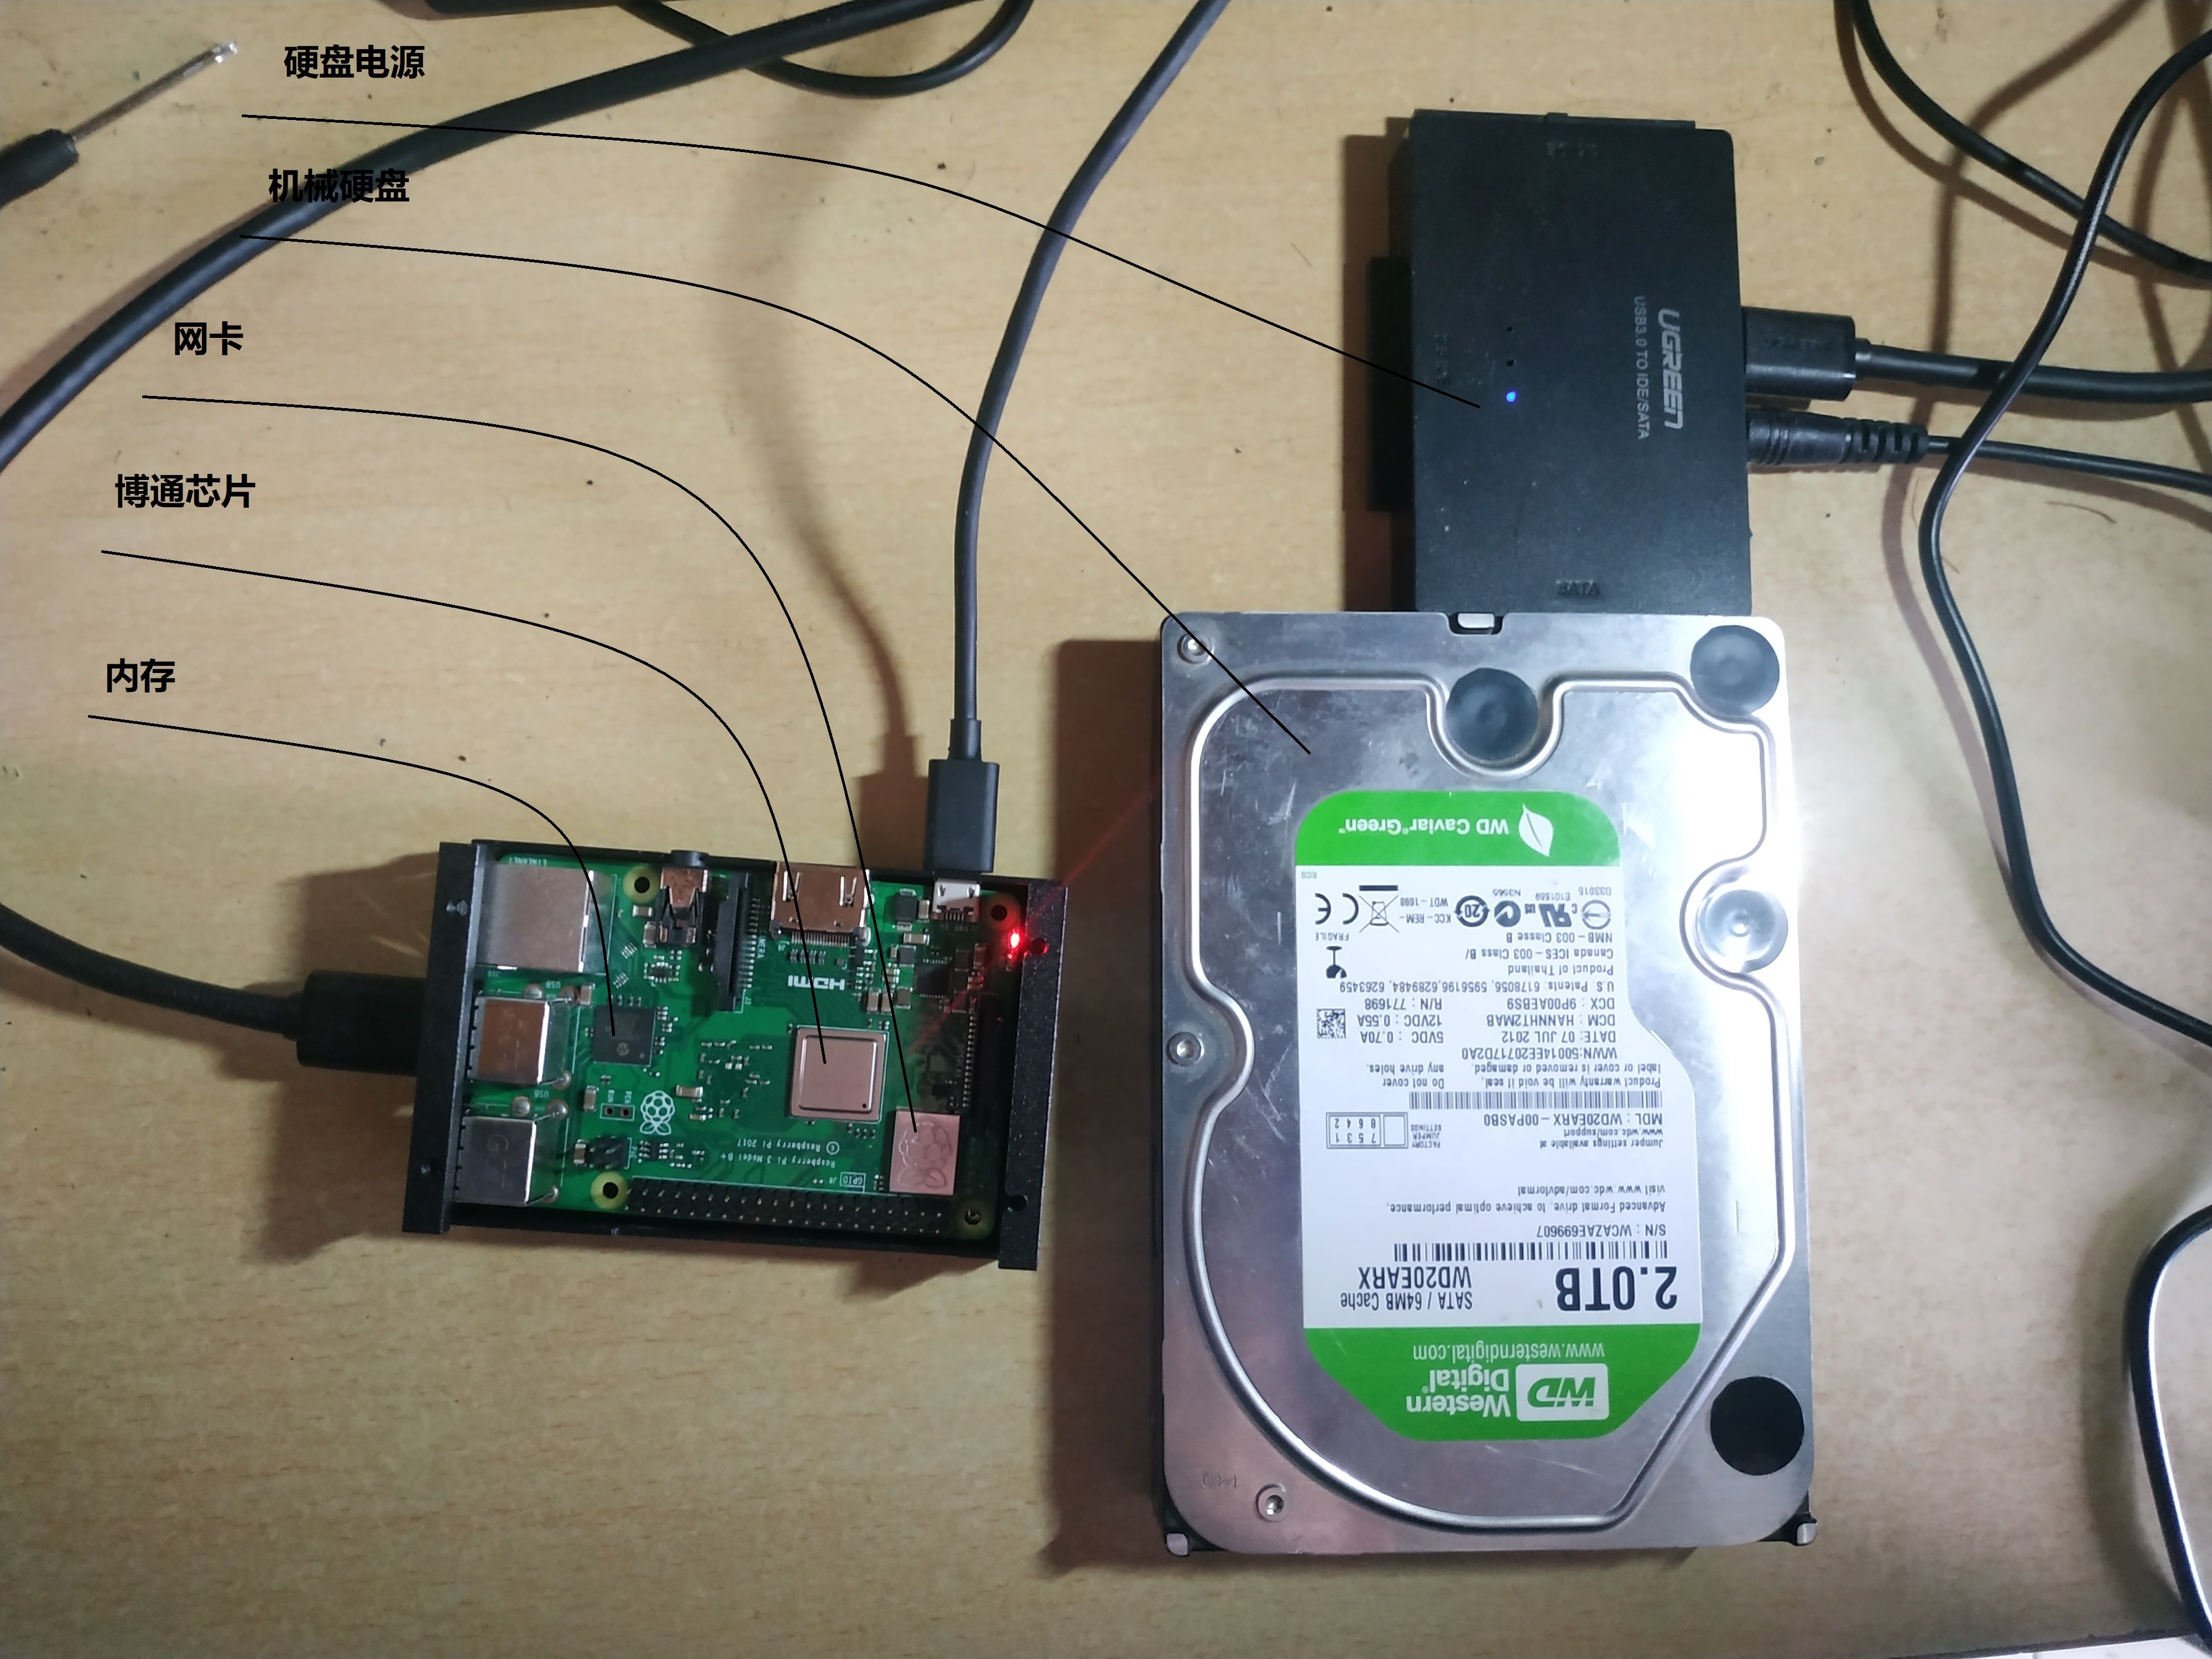
\includegraphics[width=130mm]{./figures/rasberry.jpg}
  \caption{树莓派单片机 2T硬盘}
  \label{raspberrypi}
\end{figure}


\subsection{研究背景}
\paragraph{终端存储空间不足}
对普通的个人消费者用户来说,移动手机还有个人计算机是两种比较常见的终端设备。用户在平时的工作,学习,娱乐中,
会积累下来许许多多的文件,视频,音乐,图片,文本文档,游戏,还有下载的各种资源,这些文件通常占据
了我们绝大部分的存储空间,我们电脑上的存储空间,手机上的存储空间,往往不够用,这时候大家就会想到,将这些文件备
份到云端硬盘中,为本地节省下来存储空间\cite{r7,r9,r10}。

现在市面上主流的手机存储容量一般有16G,32G,64G,128G,256G,然而对于手机用户来说,这些容量往往是不够用的。
现在的手机应用占用的存储空间非常容易能达到300MB以上,QQ微信的空间会更多一点。QQ微信微信照片内容分享,再加上现如今的如今
比较流行的短视频应用,摄像录影对用户来说可以说是绝对的刚需了。这时候一个普通的用户平时的照片视频存下来的话,
没几天消耗的存储空间都能达到上百兆,一张照片有3到5兆的大小,用手机拍摄的没有经过后期的视频一分钟都有150M左右,
很快的手机终端的存储空间被消耗殆尽。当然手机的厂家都会提供自身的云服务,但是在超过免费的存储容量之后,手机厂商
就回收取非常昂贵的云存储费用。

相比使用闪存技术来存储数据的手机来说,个人计算机一般采用128GB,或者256GB的SSD固态硬盘作系统盘,外加500GB,
或者1TB的机械硬盘来做数据存储盘。因此对电脑相对手机来说,存储设备的价格相比手机还是要低一些的,下面是一些固态
和机械硬盘的价格图标,机械硬盘的价格还是可以接受的,但是在终端设备存储数据有一个很大的弊端
就是数据的容灾不能得到保证,因为终端损坏而导致数据丢失用户后悔不及的事情屡屡发生。因此本项目数据和终端的分离就显得
非常有现实意义了。

\begin{figure}[H]
  \centering
  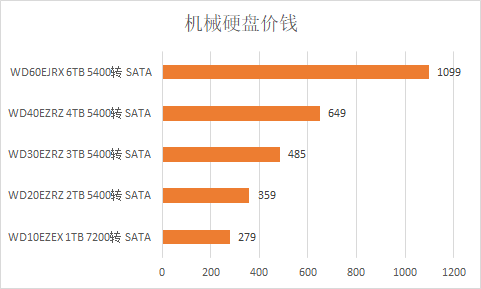
\includegraphics[width=130mm]{./figures/raid2.png}
  \caption{ 西部数据硬盘价钱\cite{r19}}
\end{figure}

\paragraph{云盘服务价格昂贵}
云存储是一项刚需,现在各手机厂商都会有自家的云存储,像苹果的icloud,小米的Mi Cloud等,但是价格并不便宜。
苹果的icloud的一年2TB的存储空间的价格为810元\cite{r22},小米10G就要收费60元,现在市场上比较流行的是百度云,
百度一开始有3TB的免费的存储空间,但是如果你额外要存储更多的数据的话,可以向他购买一年2TB价格为249元
的存储空间套餐,但是百度云对非会员用户来说下载速度有很大的限制,现在百度云将非百度云会员的下载速度限制在500KB/S以下。

国外比较流行的云存储服务,有谷歌的Google Drive,微软的One Drive,亚马逊的Amazon Cloud Driver,
但是国外的云存储服务有两个很明显的缺点,一个是价格,比百度云还要昂贵,而且因为特殊的国情这些国外的云存储厂家都没有
在国内开服务器,在网络的稳定性和速度上有很大的折扣\cite{r11,r12,r13,r14}。相比于各厂商提供的方案,本系统可以提供一种更为经济的云盘解决方案,
就是通过树莓派(英语:Raspberry Pi)和家庭宽带来部署云盘服务。闲鱼上1块2TB的二手机械硬盘,大概需要250块钱左右,
我们知道一块机械硬盘的寿命可以维持在4到5年左右,平均下来每年只需要花90多块钱就可以享受到2TB的存储空间,一个私人的云存储服务,
可以花更少的价钱而得到更大的存储空间。

\begin{figure}[H]
  \centering
  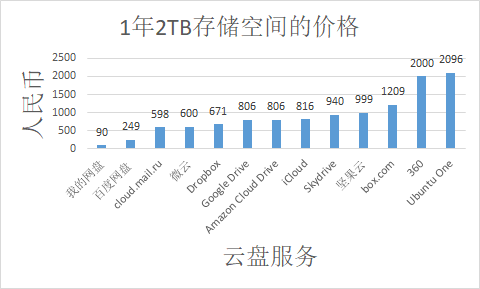
\includegraphics[width=130mm]{./figures/cloud_price.png}
  \caption{市场上主流的云盘服务价钱\cite{r11,r12,r13,r14,r22,r23}}
\end{figure}

当然私人的云盘服务有很大的缺点就是,在文件共享,异地访问,并发访问,相比于成熟的商业公司提供的云存储
服务有很大的缺陷。本项目是利用上海电信提供的20兆家庭宽带,服务器上载速度明显限制在500KB/s以下。在本项目的实验中,
在北京异地访问寝室树莓派上的视频文件只能够保证20KB/s的速度,效果不能令人满意。但是局域网环境下,本系统基本可以做到
1.25MB/s的上载下行速度。

\paragraph{家庭宽带和磁盘资源没有得到充分利用}
家庭宽带和硬盘资源很难得到充分的利用。因为学习和工作的原因,用户不在家时间占了大部分的时间,宽带资源往往得不到充分的利用。
同时因为硬盘技术的发展,旧电脑的机械硬盘被固态硬盘取代,这些淘汰下来的机械硬盘也得不到充分利用。本系统的目的之一就是开发一种
在线存储系统,将这些淘汰的资源充分利用起来。

关于使用旧的硬盘有硬盘损坏数据丢失的风险。机械硬盘的理论寿命大约三万个小时,企业级硬盘、监控用硬盘,如果始终保持高速运转工作,
三年的话就会而损坏,消费者级的硬盘正常使用6到7年是没有问题的,不过硬盘的寿命的的预测大多基于生产数据的结果统计,相关的理论分析还是很缺乏,
也没有相应的研究成果公布\cite{r24}。一般机械硬盘的寿命和它的读写数次数有关,如果频繁读写的话,机械硬盘的寿命会大大的降低,
但是本项目的磁盘独显磁盘读写的场景并不多,而且本项目还做了相对应的增量备份,异地备份,在一定程度上保证了数据安全。

\paragraph{文件增量备份、异地备份}
文件备份的重要性不言而喻,一旦发生灾难或错误操作的时候,我们需要一种手段能够有效的恢复系统的数剧。在文件备份手段方面,
有三个主要的形式,完全备份、增量备份和差异备份,如何在确保数据安全的基础上能够尽量减少存储空间的消耗,这是本系统要解决的难题。
另外,如果要确保数据的容灾,需要做到异地备份,本系统原始数据是存放在家里或者寝室中的机械硬盘中,发生数据损坏的概率很小,
但是数据的重要性是不言而喻的,所以需要做到一点在异地备份的方案中,有两个可选择的方案,一种是成
本比较低的,就是在寝室或者家中各有一个服务器进行备份,另外就是使用亚马逊的aws的s3存储服务,使用云存储的安全性更高,但相应的备份速度
更慢而且成本更高\cite{r25}。有一种方案是二者的结合,在家中和寝室的服务中进行备份的同时,有重要标签的文件使用商业公司提供的云存储服务,这是一个
安全和成本兼顾的方案了。


\subsection{本文贡献}

\subsubsection{云盘系统实现}
\par 本文实现了一个提供文件备份、共享、存储、访问、搜索、管理等功能,满足多终端使用的且部署在单片机树莓派上在线云盘存储系统。
从图\ref{total_system}可以看出树莓派体积非常小,仅有大概4英寸的大小,这意味着
它的能耗非常低。实验数据表明树莓派的平均功耗只有2W/h,意味着如果全年运行树莓派仅仅需要消耗18度电,
但是它的性能完全能够满足文件的上传备份访问、少量并发等基本功能,相比于个人计算机或者是专业的商用计算机来说,
树莓派的功耗可以说是几乎忽略不计\cite{26}。本系统通过路由器的端口映射,提供外网访问的功能,用户可以通过安卓客户端或者
web来访问存储在机械硬盘上的文件。经过测试,局域网内的文件上传能达到19.7Mbps的上载速度,20.4Mbps的下载速度。
本实验的路由器网卡速率为500Mbps,基本上满足局域网的文件访问功能。经过测试,北京访问基于上海电信网络环境
的树莓派上的文件可以达到平均25Kbps的速率,非常遗憾这个速率不能满足异地文件访问的要求。当然网速取决于运营商提供的网络套餐,
没有必要在代码上进行优化,况且本系统的使用场景大多是在寝室局域网和校园网、城域网内,所以像文件的备份和远程访问都是没问题的。
除了性能上的可用性,本系统还实现了Web客户端(图\ref{web_jiemian}、安卓客户端(图\ref{android_jiemian}),用户所需要的基本的云盘
功能都有实现,所以本系统具备功能上的可用性。
\begin{figure}[H]
  \centering
  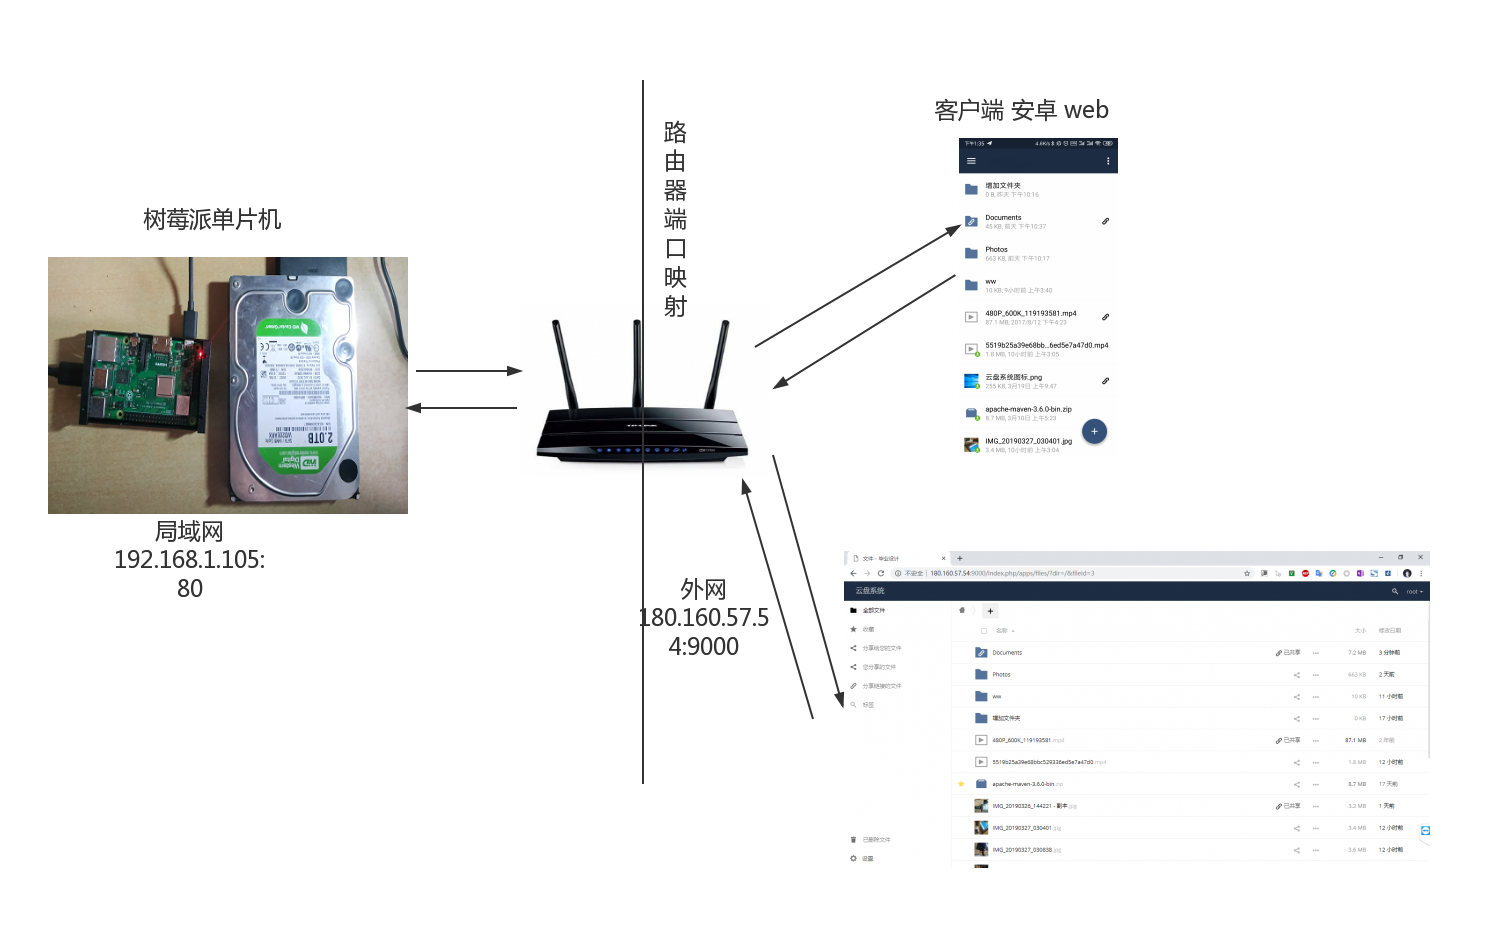
\includegraphics[width=130mm]{./figures/total_system.png}
  \caption{系统总览}
  \label{total_system}
\end{figure}

\subsubsection{Web客户端实现}
\par 本系统Web端基于jquery-ui和bootstrap实现良好的用户界面,用户可以对文件进行增删改查的操作,也可以分享文件,添加标签,
收藏文件,上传下载文件,基于html5视频在线播放,还有图片预览等功能。

\begin{figure}[H]
  \centering
  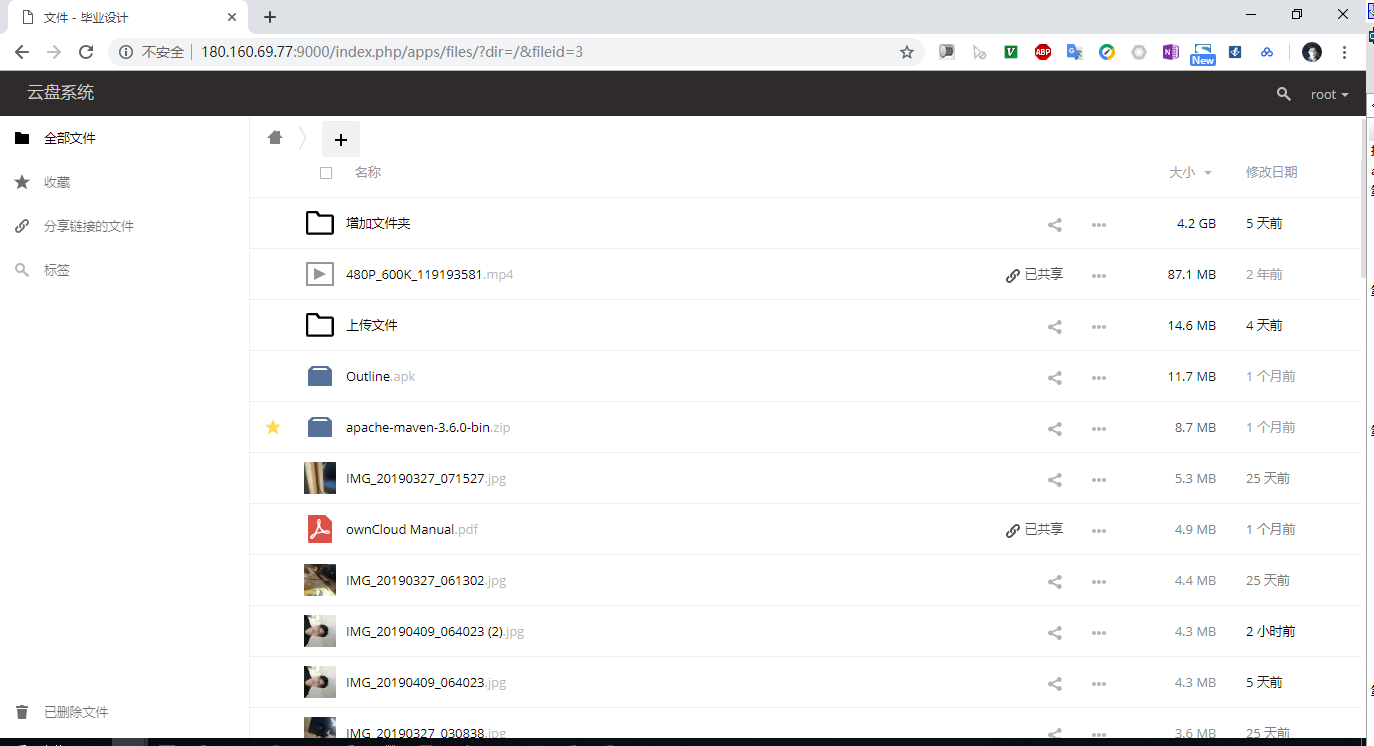
\includegraphics[width=130mm]{./figures/web1.png}
  \caption{web界面}
  \label{web_jiemian}
\end{figure}
\subsubsection{安卓客户端实现}
\par 本系统安卓端基于MaterialDrawer UI框架实现良好的用户界面,基于Volley网络框架实现文件的上传下载,手机图片视频文件
自动上传。
\begin{figure}[H]
  \centering
  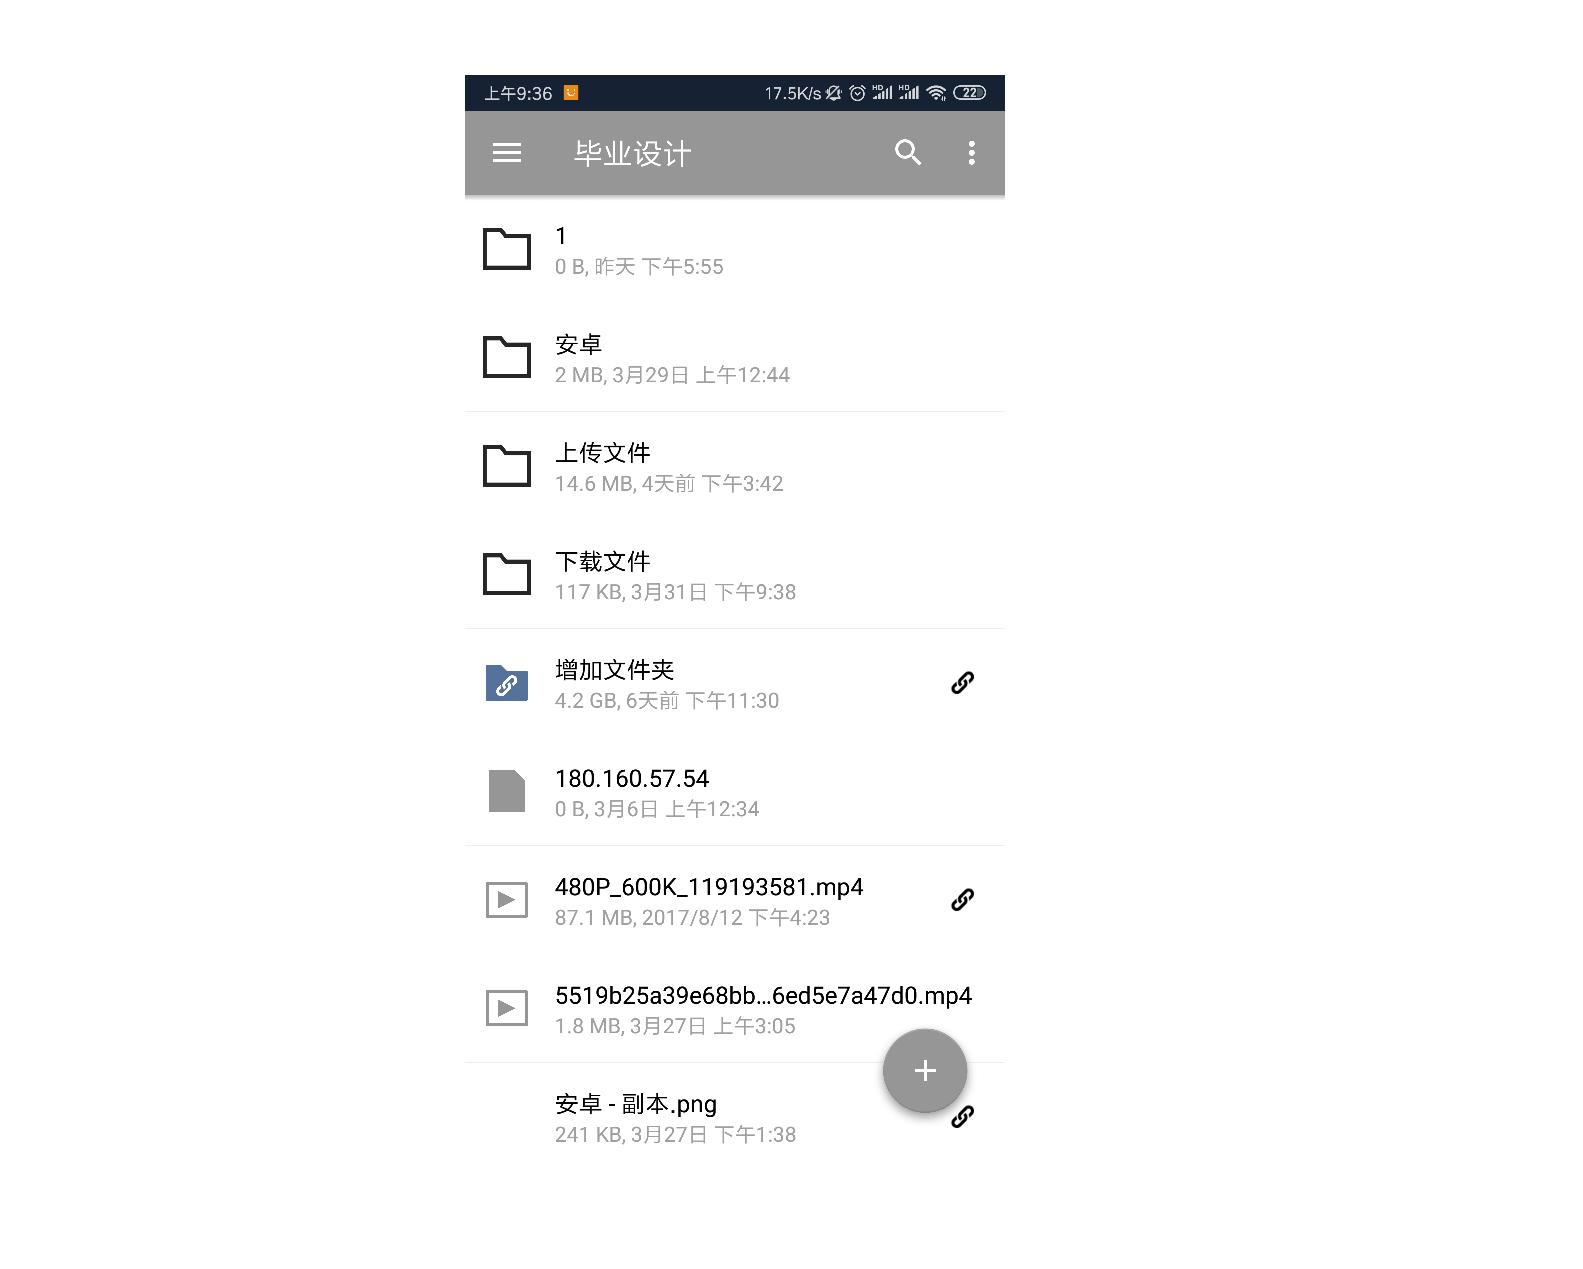
\includegraphics[width=130mm]{./figures/android2.png}
  \caption{安卓界面}
  \label{android_jiemian}
\end{figure}

\subsubsection{安卓端拍摄图片、视频自动上传}
用户可以选在开启或者关闭安卓端的文件自动备份,自动备份的原理是在安卓后台运行一个Service进程对手机/storage/emulated/0下的
目录如图\ref{android_dir}进行监听,当有新文件时会自动读取新文件,通过上传组件与服务器进行交互。因为这一个过程需要大量的后
台资源,手机端的app是默认关闭的。当然为了提升用户体验,也可以设定为在特定时间进行文字备份,比如凌晨时间。
\begin{figure}[H]
  \centering
  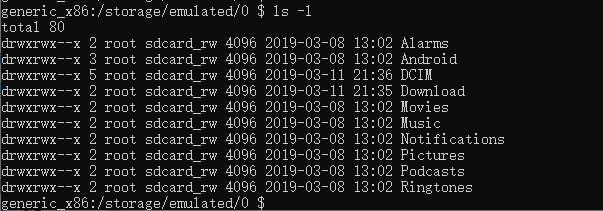
\includegraphics[width=130mm]{./figures/android_dir.png}
  \caption{需要监听的外部存储的目录}
  \label{android_dir}
\end{figure}

\subsubsection{文件增量备份、异地备份}
系统需要至少两台机器来进行文件备份,机器间需要保持数据的同步,如果数据不一致,需要快速的定位到不一致的节点。
本系统实现了在每台机器上针对每个目录数据的散列值维护一棵Merkle树,这样在两台机器间进行数据比对时,从Merkle树
的root节点开始进行比对,如果root节点一样,则表示这两台机器间的目录数据是一致的,不再需要任何处理;如果不一样,
则遍历Merkle树,定位到不一致的节点也非常快速。相比于无脑地对文件进行完全备份,使用文件的哈希值作为文件的身
份标识来构建Merkle树的做法提升了备份的速度和存储空间。

\subsubsection{文件收藏、标签、搜索}
用户可以为文件打上标签,或者收藏,系统会提供额外的分享,收藏,标签,垃圾箱目录给用户访问,用户不用取辛苦寻找标记过的文件。同时系统还提供
文件名模糊搜索(文件限定于在本目录搜索,如果采用和Windows的Exploer的深度全局查找,系统开销会非常大,而且效果不好,一般用户都会记
得特定文件的存放目录,实现文件全局查找实在没有工程上的必要),标签查找。查找结果会动态的在前端页面展示出来,用户体验非常良好。

\subsection{研究思路}
本文从需求分析、概念结构设计、逻辑结构设计、编程实现、实验验证、测试运行几个方面展开研究。
\paragraph{需求分析}
需求分析阶段要对整个云盘系统有一个清晰明确的认识,将各个需求分割成可实现的各个小模块,明确系统的使用场景和面向的使用人群,
指定开发的标准规范,名且系统的设计和实现目标,正对具体业务进行分析和差分,做好业务逻辑说明,明确系统角色,同时要明确哪些
需求是功能性需求,哪些是非功能性需求,这样才能明确重点,提高开发的效率。
\paragraph{概念结构设计、逻辑结构设计}
主要采用E-R模型进行设计,包括画E-R图,然后通过将E-R图转换成表,实现从E-R模型到关系模型的转换,再然后为所设计的数据库选择
合适的存储结构和存取路径。
\paragraph{编程实现}
选定好技术框架后就可以马上动手实现系统了。本系统的技术框架大概有PHP,Apache,MySql,jquery,jquery-ui,bootrap,Android,Volley,
MaterialDrawer UI等。
\paragraph{实验验证、测试运行}
实现主要比较在不通网络环境(局域网,广域网),异地访问,本地访问,WiFi环境,校园网环境、基站流量下对云盘系统的上传下载的速度和
稳定性等基础功能进行测试。功能性测试方面要同时完成网页端和安卓端的单元测试、集成测试、系统测试、性能测试,安全测试、兼容性、接口
测试、极限测试等。性能测试方面要完成对预期性能指标、核心模块并发、组合模块并发、大数据量、疲劳强度、网络性能等多个场景的测试。
并通过实验得到实验数据来完成对系统的可用性和安全性的验证。

\subsection{论文组织}
本文一共分为六个章节,其结构安排如下:

第一章为绪论部分。讲述了本文的研究背景,阐述了本文的研究内容和贡献,并对研究结果做了简单的展示。

第二章为系统需求分析部分。结合文件管理系统实际,分别对系统的总体性需求、功能性需求、非功能性需求、系统技术可行性等几个方面进行介绍和分析。

第三章为系统功能设计部分。在需求分析的基础上对云盘系统进行总体设计,首先介绍了系统设计的目标和原则,在基于以上原则的基础上分别对系统的服务器
架构、使用的一些技术框架,和数据库表格做了详细的介绍和分析。

第四章为系统功能实现部分。在完成功能分析和系统设计之后,此部分详细介绍展示了系统实现的结果,ui界面,系统操作步骤,和一些关键功能的算法实现。

第五章为系统测试与分析部分。此部分结合本系统的实际别对一些常见的测试方法进行粗略的介绍,同时详细介绍了本系统测试时所需要的测试环境和测试工具,
然后本文设计了一些关键的测试用例,并对测试结果进行分析和总结,最后本文用Linux工具dstat对服务器的性能进行粗略的分析。

第六章为总结与展望部分。对本文的主要工作以及创新点进行总结,对未来研究进行展望。